\documentclass[journal,12pt,onecolumn]{IEEEtran}

%--- PREAMBLE ---
% Workaround for conflict between amsmath and txfonts
\let\negmedspace\undefined
\let\negthickspace\undefined

% --- PACKAGES ---
\usepackage[utf8]{inputenc} % Modern input encoding
\usepackage[T1]{fontenc}    % Font encoding for better output
\usepackage{cite}
\usepackage{amsmath,amssymb,amsfonts,amsthm}
\usepackage{algorithmic}
\usepackage{graphicx}
\graphicspath{{./figs/}}
\usepackage{textcomp}
\usepackage{xcolor}
\usepackage{txfonts}
\usepackage{listings}
\usepackage{enumitem}
\usepackage{mathtools}
\usepackage{gensymb}
\usepackage{comment}
\usepackage{caption}
\usepackage{tkz-euclide}
\usepackage{gvv} % Note: This is a non-standard package and requires gvv.sty file
\usepackage{xparse}
\usepackage{array}
\usepackage{longtable}
\usepackage{calc}
\usepackage{multirow}
\usepackage{multicol}
\usepackage{hhline}
\usepackage{ifthen}
\usepackage{lscape}
\usepackage{tabularx}
\usepackage{float}
\usepackage[breaklinks=true]{hyperref} % Should be loaded last

% --- THEOREM DEFINITIONS & CUSTOM COMMANDS ---
\newtheorem{theorem}{Theorem}[section]
\newtheorem{problem}{Problem}
\newtheorem{proposition}{Proposition}[section]
\newtheorem{lemma}{Lemma}[section]
\newtheorem{corollary}[theorem]{Corollary}
\newtheorem{example}{Example}[section]
\newtheorem{definition}[problem]{Definition}
\theoremstyle{remark}

\begin{document}

% --- TITLE & AUTHOR ---
\title{GATE 2016 BT}
\author{EE25BTECH11014 - BHOOMIKA LOKESH}
\maketitle

% Note: The following commands change the numbering of all figures and tables
% to match the main question counter. This can be fragile.
\renewcommand{\thefigure}{\theenumi}
\renewcommand{\thetable}{\theenumi}
\begin{enumerate}


\section{Q.1-Q.5 carry one mark each}
\item The volume of a sphere of diameter 1 unit is 	  than the volume of a cube of side 1 unit.
    \begin{multicols}{4}
    \begin{enumerate}
    \item least	
    \item less
    \item lesser 
    \item low    
\end{enumerate}
\end{multicols} \hfill(GATE BT 2016)  

\item The unruly crowd demanded that the accused be 	 without trial.
  \begin{multicols}{4}
    \begin{enumerate}
    \item hanged	
    \item hanging
    \item hankering	
    \item hung
\end{enumerate}
\end{multicols} \hfill(GATE BT 2016)   

\item Choose the statement(s) where the underlined word is used correctly:
  \begin{enumerate}[label=\roman*.]
\item A prone is a dried plum.
\item He was lying prone on the floor.
\item  People who eat a lot of fat are prone to heart disease.
   \end{enumerate}
    \begin{multicols}{2}
    \begin{enumerate}
\item \brak{i} and \brak{iii} only	
\item \brak{iii} only	
\item \brak{i} and \brak{ii} only	
\item \brak{ii}and \brak{iii} only
     \end{enumerate}
     \end{multicols} \hfill(GATE BT 2016)   

\item \textbf{Fact}\:If it rains, then the field is wet.\\
Read the following statements\:
  \begin{enumerate}[label=\roman*.]
\item It rains
\item The field is not wet
\item The field is wet
\item It did not rain
 \end{enumerate}
Which one of the options given below is NOT logically possible, based on the given fact?
   \begin{multicols}{2}
    \begin{enumerate}
\item  If (iii), then (iv).	
\item If (i), then (iii).
\item If (i), then (ii).	
\item If (ii), then (iv).
     \end{enumerate}
     \end{multicols} \hfill(GATE BT 2016)  

\item A window is made up of a square portion and an equilateral triangle portion above it. The base of the triangular portion coincides with the upper side of the square. If the perimeter of the window is $6$ m, the area of the window in m$2$ is 	.
 \begin{multicols}{2}
    \begin{enumerate}
\item $1.43$
\item $2.06$
\item $2.68$	
\item $2.88$
 \end{enumerate}
     \end{multicols} \hfill(GATE BT 2016)   


 \section{Q.6-Q.10 carry one mark each}
\item Students taking an exam are divided into two groups,\textbf{ P} and \textbf{Q} such that each group has the same number of students. The performance of each of the students in a test was evaluated out of $200$ marks. It was observed that the mean of group \textbf{P} was $105$, while that of group \textbf{Q} was $85$. The standard deviation of group P was $25$, while that of group \textbf{Q} was $5$. Assuming that the marks were distributed on a normal distribution, which of the following statements will have the highest probability of being \textbf{TRUE}?
 \begin{multicols}{2}
 \begin{enumerate}
 \item No student in group\textbf{Q} scored less marks than any student in group \textbf{P}.
\item No student in group\textbf{P} scored less marks than any student in group \textbf{Q}.
\item  Most students of group \textbf{Q} scored marks in a narrower range than students in group \textbf{P}.
\item  The median of the marks of group \textbf{P} is $100$.
 \end{enumerate}
 \end{multicols} \hfill(GATE BT 2016)   
 
\item A smart city integrates all modes of transport, uses clean energy and promotes sustainable use of resources. It also uses technology to ensure safety and security of the city, something which critics argue, will lead to a surveillance state.\\ \hfill(GATE BT 2016) 

 Which of the following can be logically inferred from the above paragraph?
\begin{enumerate}[label=\roman*.]
\item All smart cities encourage the formation of surveillance states.
\item Surveillance is an integral part of a smart city.
\item Sustainability and surveillance go hand in hand in a smart city.
\item  There is a perception that smart cities promote surveillance.
\end{enumerate}
         
\begin{multicols}{2}
\begin{enumerate}
\item (i) and (iv) only	
\item  (ii) and (iii) only
\item (iv) only
\item  (i) only

\end{enumerate}
\end{multicols} \hfill(GATE BT 2016)   

\item Find the missing sequence in the letter series.\\
B, FH, LNP,
 \begin{multicols}{4}
\begin{enumerate}
\item  SUWY	
\item TUVW	
\item  TVXZ	
\item TWXZ
\end{enumerate}
\end{multicols} \hfill(GATE BT 2016)   

\item The binary operation   is defined as a   b $=$ ab$+\brak{a+b}$, where a and b are any two real numbers. The value of the identity element of this operation, defined as the number x such that a   x $=$ a, for any a, is   
\begin{multicols}{4}
\begin{enumerate}
\item $0$
\item $1$	
\item $2$
\item $10$
\end{enumerate}
\end{multicols} \hfill(GATE BT 2016)   

\item Which of the following curves represents the function $y=ln(|e^{[|sin(|x|)|]}|)$ for $|x|<2\pi$?.\\Here, x represents the abscissa and y represents the ordinate.
\begin{figure}[H]
    \centering
 \begin{multicols}{2}
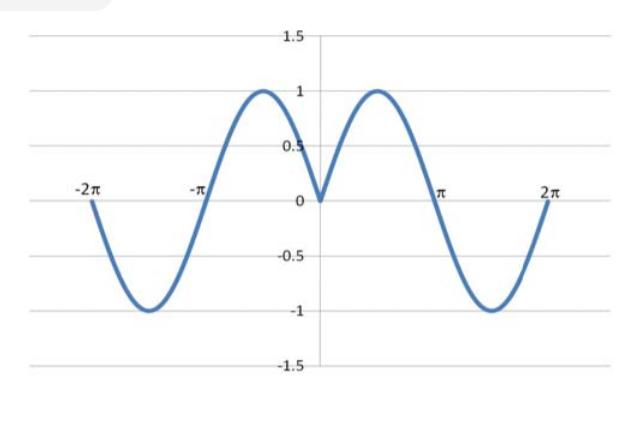
\includegraphics[width=0.7\columnwidth]{figs_2/fig_2.10.1.jpeg}
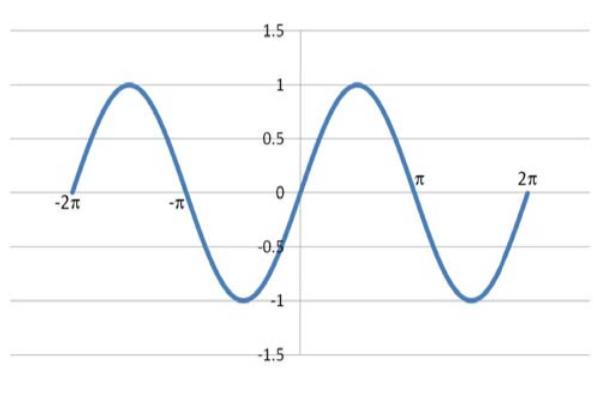
\includegraphics[width=0.7\columnwidth]{figs_2/fig_2.10.2.jpeg}
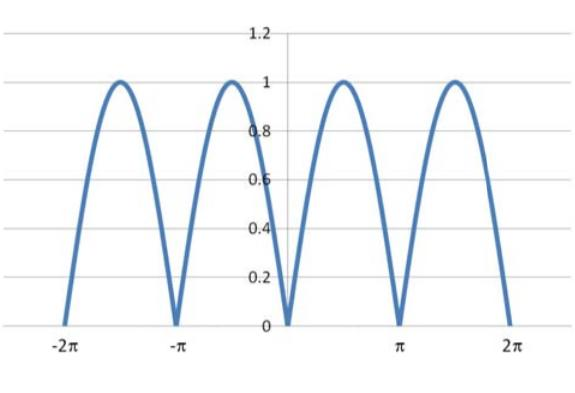
\includegraphics[width=0.7\columnwidth]{figs_2/fig_2.10.3.jpeg} 
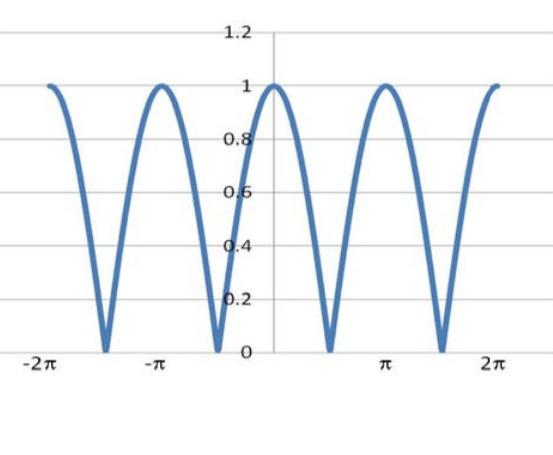
\includegraphics[width=0.7\columnwidth]{figs_2/fig_2.10.4.jpeg}
 \end{multicols} \hfill(GATE BT 2016)     
\end{figure}


\end{enumerate}

\section{Q.1-Q.25 carry one mark each}
\begin{enumerate}
  \item Bacteria with two or more flagella at one or both ends are called
\begin{multicols}{4}
\begin{enumerate}
\item amphitrichous	
\item  peritrichous	
\item  lophotrichous	
\item  atrichous
\end{enumerate}
\end{multicols} \hfill(GATE BT 2016)   

 
\item Which family of viruses has single stranded DNA?
\begin{multicols}{4}
\begin{enumerate}
\item  Herpesviridae	
\item Poxviridae	
\item Retroviridae	
\item Parvoviridae
\end{enumerate}
\end{multicols} \hfill(GATE BT 2016)  

\item What will be the binding status of regulatory proteins in lac operon when concentrations of both lactose and glucose are very low in the culture medium?
\begin{multicols}{2}
 \begin{enumerate}
 \item Only the repressor remains bound to the operator
 \item Only the cyclic AMP-Catabolic Activator Protein (cAMP-CAP) complex remains bound to the CAP binding site
\item Neither the repressor nor cAMP-CAP complex remain bound to their respective binding sites
\item Both the repressor and cAMP-CAP complex remain bound to their respective binding sites
 \end{enumerate}
\end{multicols} \hfill(GATE BT 2016)  

\item Which of the following are TRUE for Treponema pallidum?\\
    P. It is the causative agent of syphilis\\
    Q. It is a spirochete\\
    R. It is a non-motile bacterium\\
    S. It is generally susceptible to penicillin\\
Choose the correct combination.
\begin{multicols}{4}
\begin{enumerate}
\item  P, Q and R only
\item P, Q and S only	
\item P, R and S only	
\item Q, R and S only
\end{enumerate}
\end{multicols} \hfill(GATE BT 2016)  

\item In a typical mitotic cell division cycle in eukaryotes, M phase occurs immediately after the
\begin{multicols}{4}
\begin{enumerate}
\item $G_0$ phase	
\item S phase
\item $G_1$ phase	
\item $G_2$ phase
\end{enumerate}
\end{multicols} \hfill(GATE BT 2016)  

\item Which one of the following is NOT a therapeutic agent based on nucleic acid for the treatment of genetic disorders?
\begin{multicols}{2}
\begin{enumerate}
\item Antisense oligonucleotide	
\item Ribozyme
\item Aptamer
\item Avidin
\end{enumerate}
\end{multicols} \hfill(GATE BT 2016)   

\item ATP biosynthesis takes place utilizing the H+ gradient in mitochondria and chloroplasts. Identify the correct sites of H+ gradient formation.
\begin{multicols}{2}
\begin{enumerate}
\item  Across the outer membrane of mitochondria and across the inner membrane of chloroplast
\item  Across the inner membrane of mitochondria and across the thylakoid membrane of chloroplast
\item  Within the matrix of mitochondria and across the inner membrane of chloroplast
\item  Within the matrix of mitochondria and within the stroma of chloroplast
\end{enumerate}
\end{multicols} \hfill(GATE BT 2016)   

\item Which one of the following is NOT an algorithm for building phylogenetic trees?
\begin{multicols}{2}
\begin{enumerate}
\item Maximum parsimony	
\item Neighbor joining
\item  Maximum likelihood	
\item  Bootstrap
\end{enumerate}
\end{multicols} \hfill(GATE BT 2016)  

\item Cesium chloride density gradient centrifugation is commonly used for the separation of DNA molecules. The buoyant density, $\rho$, of a double stranded $Cs^+$ DNA is given by the equation $\rho$$= 1.66 + 0.098X_{G+C}$
where $X_{G+C}$ denotes
\begin{multicols}{2}
\begin{enumerate}
\item total number of G and C	
\item  mole fraction of G$+$C
\item  number of GC repeats	
\item ratio of G$+$C to A$+$T content
\end{enumerate}
\end{multicols} \hfill(GATE BT 2016)  

\item Disaccharide molecules that contain $\beta$ ($1\rightarrow 4$) glycosidic linkage are
\begin{multicols}{2}
\begin{enumerate}
\item sucrose and maltose	
\item  sucrose and isomaltose
\item maltose and isomaltose
\item lactose and cellobiose
\end{enumerate}
\end{multicols} \hfill(GATE BT 2016)   

\item  Junctional diversity of antibody molecules results from
 \begin{multicols}{2}
\begin{enumerate}
\item the addition of switch region nucleotides
\item the addition of N and P nucleotides
\item  the joining of V, D and J segments
\item  mutations in complementarity-determining regions
\end{enumerate}
\end{multicols} \hfill(GATE BT 2016)  

\item  Which one of the following is \textbf{ NOT} used for the measurement of cell viability in animal cell culture?
\begin{multicols}{2}
\begin{enumerate}
\item Trypan blue dye exclusion
\item Tetrazolium (MTT) assay
\item LDH activity in the culture medium
\item Coulter counter
\end{enumerate}
\end{multicols} \hfill(GATE BT 2016)  

\item Which one of the following techniques relies on the spin angular momentum of a photon?
\begin{multicols}{2}
\begin{enumerate}
\item CD spectroscopy	
\item Fluorescence spectroscopy
\item IR spectroscopy	 
\item Raman spectroscopy
\end{enumerate}
\end{multicols} \hfill(GATE BT 2016)   


\item  Which one of the following statements is \textbf{NOT} true?
\begin{enumerate} 
\item In competitive inhibition, substrate and inhibitor compete for the same active site of an enzyme
 \item  Addition of a large amount of substrate to an enzyme cannot overcome uncompetitive inhibition
 \item  A transition state analogue in enzyme catalyzed reaction increases the rate of product formation
\item  In non-competitive inhibition, Km of an enzyme for its substrate remains constant as the concentration of the inhibitor increases
\end{enumerate}\hfill(GATE BT 2016) 

\item  Based on their function, find the \textbf{ODD} one out.
\begin{multicols}{4}
\begin{enumerate}
\item miRNA	
\item siRNA	
\item shRNA	
\item snRNA
\end{enumerate}
\end{multicols} \hfill(GATE BT 2016)   

\item Prandtl number is the ratio of
\begin{multicols}{2}
\begin{enumerate}
\item thermal diffusivity to momentum diffusivity
 \item  mass diffusivity to momentum diffusivity
\item  momentum diffusivity to thermal diffusivity
\item  thermal diffusivity to mass diffusivity
\end{enumerate} \end{multicols}
\hfill(GATE BT 2016) 

\item  Fed batch cultivation is suitable for which of the following?\\
P. Processes with substrate inhibition\\
Q. Processes with product inhibition\\
R. High cell density cultivation
\begin{multicols}{4}
\begin{enumerate}
\item P and Q only	
\item P and R only	
\item Q and R only	
\item  P, Q and R
\end{enumerate}
\end{multicols} \hfill(GATE BT 2016) 

\item A biological process is involved in the \rule{3cm}{0.4pt}
treatment of industrial effluent.
\begin{multicols}{4}
\begin{enumerate}
\item  primary
\item  secondary
\item  tertiary
\item quaternary
\end{enumerate}
\end{multicols} \hfill(GATE BT 2016)   

\item In dead-end filtration, rate of filtration is
\begin{multicols}{2}
\begin{enumerate}
\item directly proportional to the square root of pressure drop across the filter medium
\item  inversely proportional to the pressure drop across the filter medium
\item inversely proportional to the viscosity of the solution
\item  inversely proportional to the square of viscosity of the solution

\end{enumerate}
\end{multicols} \hfill(GATE BT 2016)  

\item The power required for agitation of non-aerated medium in fermentation is\rule{2cm}{0.4pt} kW. Operating conditions are as follows:\\

Fermentor diameter $= 3$ m\\ Number of impellers $= 1$ \\Mixing speed $= 300$ rpm\\
Diameter of the Rushton turbine $= 1$ m \\Viscosity of the broth $= 0.001$ Pa.s \\Density of the broth $= 1000 kg.m{-3}$\\ Power number $= 5$  \hfill(GATE BT 2016)  

\item Which one of the following is the most suitable type of impeller for mixing high viscosity (viscosity $> 10^{5}$ cP) fluids?
\begin{multicols}{4}
\begin{enumerate}
\item  Propeller	
\item  Helical ribbon	
\item  Paddle 
\item  Flat blade turbine
\end{enumerate}
\end{multicols} \hfill(GATE BT 2016)   

\item  Runs scored by a batsman in five one-day matches are $55$,$ 75$, $67$, $88$ and $15$. The standard deviation is \rule{2cm }{0.4pt}  \hfill(GATE BT 2016) 	.

\item  The \textbf{positive} Eigen value of the following matrix is \rule{2cm }{0.4pt}.\\
\[
\begin{bmatrix}
  2 & 1\\5 & 2
\end{bmatrix}\] 
\hfill(GATE BT 2016) 

\item The Laplace transform \textit{F(s)} of the function f(t) = cos (at), where a is constant, is \rule{2cm }{0.4pt} 	
\begin{multicols}{4}
\begin{enumerate}
\item $\dfrac{s^{2}}{s^{2}+a^{2}}$
\item $\dfrac{a}{s^{2}+a^{2}}$
\item $\dfrac{s}{s^{2}+a^{2}}$
\item $\dfrac{s}{s^{2}-a^{2}}$
\end{enumerate}
\end{multicols} \hfill(GATE BT 2016)  

\item The value of the integral$\int_{0}^{0.9}{\dfrac{1}{(2-x)(1-x)}}\,dx$ is \rule{2cm }{0.4pt}

\section{Q.26-Q.55 carry one mark each}

\item Which combination of the following statements is \textbf{ CORRECT} for cyanobacteria?\\
P. They can perform oxygenic photosynthesis
Q. Usually filamentous forms are involved in nitrogen fixation
R. Nitrogen fixation occurs in heterocysts
S. They cannot grow in a mineral medium exposed to light and air
\begin{multicols}{4}
\begin{enumerate}
\item  P, Q and R
\item  P, S and R
\item  Q, R and S
\item P, Q and S
\end{enumerate}
\end{multicols} \hfill(GATE BT 2016)  

\item Which set of the following events occurs during the elongation step of translation?\\
P. Attachment of mRNA with the smaller subunit of ribosome\\
Q. Loading of correct aminoacyl-tRNA into the A site\\
R. Formation of a peptide bond between the amino acyl-tRNA in the A site and the peptide\\
chain that is attached to the peptidyl-tRNA in the P site\\
S. Dissociation of the ribosomal subunits\\
T. Translocation of peptidyl-tRNA from the A site to the P site of the ribosome

\begin{multicols}{4}
\begin{enumerate}
\item P, Q and R
\item  P, Q and T
\item  Q, R and T
\item  R, S and T
\end{enumerate}
\end{multicols} \hfill(GATE BT 2016)  

\item A DNA sequence, $5$’-ATGGACGTGCTTCCCAAAGCATCGGGC-$3’$, is mutated to obtain\\
P. $5’$-ATGGACGTGCTTC\textbf{a}CAAAGCATCGGGC-$3’$\\
Q. $5’$-ATGGACGTGCTTCCC\textbf{g}AAAGCATCGGGC-$3’$\\
R. $5’$-ATGGACGTGCTTCC-AAAGCATCGGGC-$3’$\\
S. $5’$-ATGGACGTGCTTCCCAA\textbf{t}GCATCGGGC-$3’$\\
T. $5’$-ATGGACG\textbf{a}GCTTCCCAAAGCATCGGGC-$3’$\\
(Point mutations are shown in the \textbf{lower case} or ‘-’ within the sequences)\\
Which of the above mutant sequences \textbf{DO NOT} have frame-shift?
\begin{multicols}{4}
\begin{enumerate}
\item P, Q and S
\item P, S and T
\item Q, R and S
\item  Q, S and T
\end{enumerate}
\end{multicols} \hfill(GATE BT 2016)  

\item  Which of the following events occur during the stationary phase of bacterial growth?\\
    P. Rise in cell number stops\\
    Q. Spore formation in some Gram-positive bacteria such as Bacillus subtilis\\
    R. Cell size increases in some Gram-negative bacteria such as Escherichia coli\\
    S. Growth rate of bacterial cells nearly equals their death rate\\
    T. Decrease in peptidoglycan crosslinking
\begin{multicols}{4}
\begin{enumerate}
\item P, Q and S only	
\item P, S and T only
\item Q, R and S only	
\item P, R and T only
\end{enumerate}
\end{multicols} \hfill(GATE BT 2016)  

\item Select the \textbf{CORRECT} combination of genetic components that are essential for the transfer of T- DNA segment from \textit{Agrobacterium tumefaciens} to plant cells.
 \begin{multicols}{2}
\begin{enumerate}
\item Border repeat sequences and oncogenes	
\item Border repeat sequences and vir genes
\item Opine biosynthetic genes and vir genes
\item Opine biosynthetic genes and oncogenes
\end{enumerate}
\end{multicols} \hfill(GATE BT 2016)  

\item Match the secondary metabolites (Column-I) with the corresponding plant species (Column-II).
\begin{tabular}{p{5cm} p{5cm}}
\textbf{Column I} & \textbf{Column II} \\
 P. Morphine	&1. Datura stramonium\\
    Q. Pyrethrins	&2. Catharanthus roseus\\
    R. Scopolamine	&3. Papaver somniferum\\
    S. Vincristine	&4. Tagetes erecta\\
\end{tabular}

\begin{multicols}{4}
\begin{enumerate}
\item P-4, Q-3, R-1, S-2	
\item  P-3, Q-4, R-1, S-2
\item P-2, Q-3, R-4, S-1	
\item P-4, Q-1, R-2, S-3
\end{enumerate}
\end{multicols} \hfill(GATE BT 2016)   


\item A variety of genetic elements are used in the transgenic plant research. Match the genetic elements (Column-I) with their corresponding source (Column-II).

\begin{tabular}{p{5cm} p{5cm}}
\textbf{Column I} & \textbf{Column II} \\

    P. Ubiquitin1 promoter	&1. Agrobacterium tumefaciens\\
    Q. Nos transcriptional terminator	&2. Streptomyces hygroscopicus\\
    R. bar selection marker gene	&3. Escherichia coli\\
    S. gus reporter gene	&4. Zea mays\\
\end{tabular}
\begin{multicols}{4}
\begin{enumerate}
\item P-2, Q-1, R-3, S-4	
\item  P-2, Q-3, R-4, S-1
\item  P-3, Q-4, R-1, S-2	
\item  P-4, Q-1, R-2, S-3
\end{enumerate}
\end{multicols} \hfill(GATE BT 2016)  

\item Match the type of chromosomal inheritance $\brak{Column-I}$ with the corresponding genetic disease or trait \brak{Column-II}.

\begin{tabular}{p{5cm} p{5cm}}
\textbf{Column I} & \textbf{Column II} \\
   
    P. Autosomal recessive inheritance	&1. Huntington disease\\
    Q. Autosomal dominant inheritance	&2. Hairy ears\\
    R. X-linked inheritance	&3. Cystic fibrosis\\
    S. Y-linked inheritance	&4. Hemophilia\\
\end{tabular}
\begin{multicols}{4}
\begin{enumerate}
\item P-1, Q-4, R-3, S-2	
\item  P-4, Q-3, R-2, S-1
\item  P-3, Q-1, R-4, S-2
\item  P-4, Q-2, R-3, S-1
\end{enumerate}
\end{multicols} \hfill(GATE BT 2016)   

\item A crossing was performed between the genotypes  \textbf{\textit{DdEeFfgg}} and\textbf{\textit{ ddEeFfGg}}. Assuming that the allelic pairs of all genes assort independently, the proportion of progeny having the genotype \textbf{\textit{ddeeffgg}} is expected to be\rule{3cm}{0.4pt}	\%.

\item The equilibrium potential of a biological membrane for$ Na^{+}$ is $55$ mV at $37$ $^\circ\mathrm{C}$. Concentration of
$Na^{+}$inside the cell is $20$ mM. Assuming the membrane is permeable to Na+ only, the Na+
concentration outside the membrane will be \rule{3cm}{0.4pt} mM.
(Faraday constant: $23062 cal.V^{-1}$ .$mol^ {-1}$ , Gas constant: $1.98 cal.mol^{-1} .K^{-1}$ ) \hfill(GATE BT 2016) 

\item A $1.2$ kb DNA fragment was cloned into BamHI and EcoRI sites located on a $2.8$ kb cloning vector. The BamHI and EcoRI sites are adjacent to each other on the vector backbone. The vector contains an XhoI site located 300 bp upstream of the BamHI site. An internal XhoI site is present in the gene sequence as shown in the figure. The resultant recombinant plasmid is digested with EcoRI and XhoI and analyzed through 1\% agarose gel electrophoresis. Assuming complete digestion with EcoRI and XhoI, the DNA fragments (in base pairs) visible on the agarose gel will correspond to:

\begin{figure}[H]
    \centering
    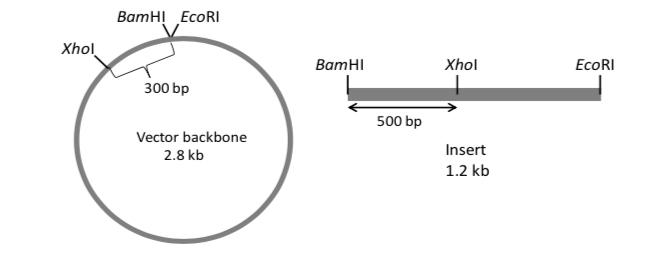
\includegraphics[width=0.7\columnwidth]{figs_2/fig_2.36.jpeg}
    \caption{figure}
    \label{fig:figure}
\end{figure}

\begin{multicols}{2}
\begin{enumerate}
\item 2800, 700 and 500	
\item 2800, 700 and 800
\item  2500, 700 and 800	
\item  2500, 1200 and 300
\end{enumerate}
\end{multicols} \hfill(GATE BT 2016) 


\item  Find the \textbf{INCORRECT} combination.

\begin{enumerate}
\item Surface immunoglobulins-B cell antigen receptor
\item Affinity maturation-isotype switching
\item Fc region of antibodies-binding to complement proteins
\item Spleen, the secondary lymphoid organ$-o$connection with the lymphatic system
\end{enumerate} \hfill(GATE BT 2016) 


\item Which of the following statement(s) is/are \textbf{CORRECT} for antigen activated effector T cells?\\
P. CD4+ cells make contact with macrophages and stimulate their microbicidal activity\\
Q. CD4+ cells make contact with B cells and stimulate them to differentiate into plasma cells\\
R. CD8+ cells make contact with B cells and stimulate them to differentiate into plasma cells\\
S. CD8+ cells make contact with virus infected cells and kill them
\begin{multicols}{4}
\begin{enumerate}
\item Q only	
\item Q and S only	
\item P, Q and S only	
\item P, Q, R and S
\end{enumerate}
\end{multicols} \hfill(GATE BT 2016)  

\item Which one of the following statements regarding G proteins is \textbf{INCORRECT}?
\begin{multicols}{2}
\begin{enumerate}
\item GDP is bound to G protein in the resting stage
\item  GTP bound  subunit cannot reassemble with  dimer
\item  All G proteins are trimeric
\item  Activation of G protein may result in activation or inhibition of the target enzymes
\end{enumerate}
\end{multicols} \hfill(GATE BT 2016)  

\item In animal cell culture, a $CO_2$ enriched atmosphere in the incubator chamber is used to maintain the culture pH between $6.9$ and $7.4$. Which one of the following statements is CORRECT?
\begin{enumerate}
 \item Higher the bicarbonate concentration in the medium, higher should be the requirement of gaseous $CO_2$
\item  Lower the bicarbonate concentration in the medium, higher should be the requirement of gaseous $CO_2$
\item  Higher the bicarbonate concentration in the medium, lower should be the requirement of gaseous $CO_2$
\item $CO_2$ requirement is independent of bicarbonate concentration in the medium
\end{enumerate}  \hfill(GATE BT 2016) 

\item Choose the \textbf{CORRECT} combination of True (T) and False (F) statements about microcarriers used in animal cell culture.\\
    P. Higher cell densities can be achieved using microcarriers\\
    Q. Microcarriers increase the surface area for cell growth\\
    R. Microcarriers are used for both anchorage- and nonanchorage-dependent cells\\
    S. Absence of surface charge on microcarriers enhances attachment of cells\\
\begin{multicols}{2}
\begin{enumerate}
\item  P-T, Q-F, R-T and S-F	
\item  P-T, Q-T, R-F and S-F
\item  P-F, Q-F, R-T and S-T	
\item  P-F, Q-T, R-F and S-T
\end{enumerate}
\end{multicols} \hfill(GATE BT 2016) 

\item In an assay of the type II dehydroquinase of molecular mass 18 kDa, it is found that the Vmax of the enzyme is $0.0134$ $\mu$mol.$min^{-1}$ when $1.8 \mu$g enzyme is added to the assay mixture. If the Km for the substrate is $25 \mu$M, the $k_{cat}/K_{m}$ ratio will be\rule{2cm}{0.4pt} 	×$104 M^{-1}.s^{-1}$. \hfill(GATE BT 2016) 


\item The molar extinction coefficients of Trp and Tyr at $280$ nm are $5690$ and $1280 M^{-1}.cm^{-1}$, respectively. The polypeptide chain of yeast alcohol dehydrogenase (37 kDa) contains 5 Trp and $14$ Tyr residues. The absorbance at $280$ nm of a $0.32 mg.mL^{-1}$ solution of yeast alcohol dehydrogenase measured in a cuvette of $1$ cm pathlength will be\rule{2cm}{0.4pt} 	.
\brak{Assume that the molar extinction coefficient values for Trp and Tyr apply to these amino acids in the yeast alcohol dehydrogenase}. \hfill(GATE BT 2016) 

\item The activity of lactate dehydrogenase can be measured by monitoring the following reaction:\\
\begin{center}$
Pyruvate + NADH\longrightarrow Lactate + NAD^{+}$\\
\end{center}
The molar extinction coefficient of NADH at $340$ nm is $6220 M^{-1}.cm^{-1}$. $NAD^{+}$ does not absorb at this wavelength. In an assay,$ 25$ $\mu$L of a sample of enzyme (containing $5 \mu$g protein per mL) was added to a mixture of pyruvate and NADH to give a total volume of 3 mL in a cuvette of $1$ cm pathlength. The rate of decrease in absorbance at $340$ nm was $0.14 min^{-1}$. The specific activity of the enzyme will be \rule{2cm}{0.4pt}	 $\mu mol.min^{-1}.mg^{-1}$. \hfill(GATE BT 2016) 

\item Analysis of a hexapeptide using enzymatic cleavage reveals the following result:\\

\textbullet Amino acid composition of the peptide is: 2R, A,V, S, Y\\
\textbullet  Trypsin digestion yields two fragments and the compositions are: \brak{R, A, V} and \brak{R, S, Y}\\
\textbullet  Chymotrypsin digestion yields two fragments and the compositions are: \brak{A, R, V, Y} and \brak{R, S}\\
\textbullet Digestion with carboxypeptidase A yields no cleavage product.\\

Given:	Trypsin cleaves at carboxyl side of R. Chymotrypsin cleaves at carboxyl side of Y.
Carboxypeptidase A cleaves at amino side of the C-terminal amino acid (except R and K) of the peptide.\\
The correct amino acid sequence of the peptide is:
\begin{multicols}{4}
\begin{enumerate}
\item RSYRVA	
\item AVRYSR	
\item SRYVAR	
\item SVRRYA
\end{enumerate}
\end{multicols} \hfill(GATE BT 2016)  

\item  The empirical formula for biomass of an unknown organism is $CH_{1.8}O_{0.5}N_{0.2}$. To grow this organism, ethanol $C_{2}H_{5}OH$ and ammonia are used as carbon and nitrogen sources, respectively. Assume no product formation other than biomass. To produce $1$ mole of biomass from $1$ mole of ethanol, the number of moles of oxygen required will be \rule{2cm}{0.4pt}.


\item  Saccharomyces cerevisiae is cultured in a chemostat (continuous fermentation) at a dilution rate of
$0.5 h^{-1}$. The feed substrate concentration is $10 g.L^{-1}$. The biomass concentration in the chemostat at steady state will be  \rule{2cm}{0.4pt} $g.L^{-1}$.\\
Assumptions: Feed is sterile, maintenance is negligible and maximum biomass yield with respect to substrate is $0.4$ (g biomass per g ethanol).
Microbial growth kinetics is given by \[ \mu = \frac{\mu_m s}{K_s+S}\]

where $\mu$ is specific growth rate \brak{h}, $\mu$m $= 0.7 h^{-1}$, Ks $= 0.3 g.L^{-1}$ and s is substrate concentration
$g.L^{-1}$ \hfill(GATE BT 2016) 

\item Decimal reduction time of bacterial spores is 23 min at $121^\circ C$ and the death kinetics follow first
order. One liter medium containing $10^5$ spores per mL was sterilized for 10 min at $121^\circ C$ in a batch sterilizer. The number of spores in the medium after sterilization (assuming destruction of spores in heating and cooling period is negligible) will be \rule{2cm }{0.4pt}×$10^7$. \hfill(GATE BT 2016) 


\item bioreactor is scaled up based on equal impeller tip speed. Consider the following parameters for small and large bioreactors\:

\begin{center}
\begin{tabular}{|c|c|c|}
\textbf{Parameters} & \textbf{Small bioreactor} & \textbf{Large bioreactor} \\
Impeller speed & $N_1$ & $N_2$ \\
Diameter of impeller & $D_1$ & $D_2$ \\
Power consumption & $P_1$ & $P_2$ \\
\end{tabular}
\end{center}
Assuming geometrical similarity and the bioreactors are operated in turbulent regime, what will be
P2/P1?
\begin{multicols}{4}
\begin{enumerate}
\item $(D_1/D_2)^2$
\item $(D_2/D_1)^2$
\item $(D_1/D_2)^5$
\item $(D_2/D_1)^5$
\end{enumerate}\end{multicols} \hfill(GATE BT 2016)  

\item An enzyme converts substrate A to product B. At a given liquid feed stream of flow rate $25 L.min^{-1}$
and feed substrate concentration of $2 mol.L^{-1}$, the volume of continuous stirred tank reactor needed
for 95\% conversion will be \rule{2cm}{0.4pt}.\\
Given the rate equation:\\
$-r_A=\dfrac{0.1C_A}{1+0.5C_A}$\\
where $- r_A$ is the rate of reaction in $mol.L^{-1}.min^{-1}$ and CA is the substrate concentration in $mol.L^{-1}$
Assumptions: Enzyme concentration is constant and does not undergo any deactivation during the
reaction. \hfill(GATE BT 2016) 

\item A protein is to be purified using ion-exchange column chromatography. The relationship between
HETP (Height Equivalent to Theoretical Plate) and the linear liquid velocity of mobile phase is
given by:

where H is HETP (m) and u is linear liquid velocity of mobile phase ($m.s^{-1}$). The values of A, B and
C are $3\times10^{-8} m^2.s^{-1}$, $3$ s and $6\times10^{-5}$ m, respectively. The number of theoretical plates based on \textbf{minimum} HETP for a column of $66$ cm length will be \rule{2cm}{0.4pt}. \hfill(GATE BT 2016) 

\item An enzyme is immobilized on the surface of a \textbf{non-porous} spherical particle of $2$ mm diameter. The
immobilized enzyme is suspended in a solution having bulk substrate concentration of $10$ mM. The
enzyme follows first order kinetics with rate constant 10 s-1 and the external mass transfer
coefficient is $1 cm.s^{-1}$. Assume steady state condition wherein rate of enzyme reaction $\brak{mmol.L^{-1}.s^{-1}}$
at the surface is equal to mass transfer rate $\brak{mmol.L^{-1}.s^{-1}}$. The substrate concentration at the surface
of the immobilized particle will be\rule{2cm}{0.4pt} mM. \hfill(GATE BT 2016) 

\item  $\dfrac{d^2y}{dx^2}-y=0$. The initial conditions for this second order homogeneous differential equation are y(0) and $\dfrac{dy}{dx}=3$ at $x=0$.
The value of y when x = 2 is\rule{2cm}{0.4pt} \hfill(GATE BT 2016) \\

\item The value of the determinant A given below is \rule{2cm}{0.4pt}.\\
A=\myvec{5 & 16 & 81\\
         0 & 2 & 2\\
         0 & 0 & 16 } \hfill(GATE BT 2016) 

\item Consider the equation\\ $V=\dfrac{aS}{b+S+\frac{S^2}{c}}$
\\Given $a=4,b=1$ and $c=9$,the \textbf{positive} value of S at which V is maximum, will be \rule{2cm}{0.4pt}. \hfill(GATE BT 2016) 

\centering
\textbf{END OF THE QUESTION PAPER}
\end{enumerate}

\end{document}

